\section{The Case for Out-of-Place Writes}\label{sec:oop}
We begin by reviewing SSD mechanics and WA, which influence both endurance and throughput.
We then argue that the DBMS is best positioned to manage end-to-end WAF at the highest layer.
To do so, however, requires adopting out-of-place writes, enabling the DBMS to use workload knowledge and SSD internals to reshape write patterns and thereby minimize flash writes per operation.

\module{Background: SSD endurance and write amplification.}
Flash SSDs differ from disks in two properties that matter for write-heavy workloads~\cite{DBLP:journals/pvldb/LeeAL23,flash-erase}.
First, flash cells only endure a limited number of program/erase cycles; each write gradually wears the cells, so device lifetime is tied to the \emph{volume of physical writes}~\cite{lerner2024principles,DBLP:conf/fast/YadgarYS15,dtp}.
Second, SSDs exhibit \emph{write amplification} because writes are performed at the page level (4-16~KiB), whereas erases reclaim entire blocks (many pages).
When a block containing still-valid pages must be erased to free space, 
the SSD first relocates those pages, increasing internal physical writes relative to host writes~\cite{DBLP:journals/pvldb/KakaraparthyPPK19,DBLP:journals/jsa/ImS10}.
Consider a DBMS issuing a write request for page $P$, as illustrated in the figure:
\begin{center}
  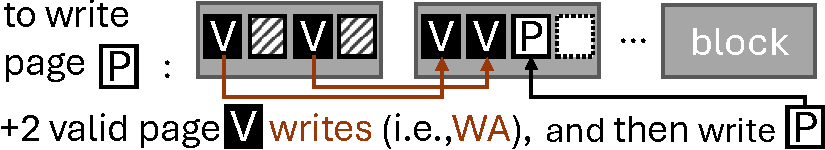
\includegraphics[clip, width=0.66\columnwidth]{figures/wa.pdf}
\end{center}
To free space, the SSD’s garbage collector selects the first block in the figure as a victim; 
because two pages in that block remain valid, it copies them elsewhere before erasing the block.
Thus, one logical write of page $P$ results in three physical writes, directly reducing SSD lifespan and the bandwidth available to the host.

\module{DB WAF: User writes transformed by the DBMS.}
To understand more about the source of WAs in \cref{fig:intro}, we first examine the DBMS write path.
The DBMS persists a safe page copy before overwriting the target~\cite{mysql-dwb,postgresql/doc/dwb}, a mechanism known as \emph{doublewrite buffering} (DWB).
For this reason, in-place systems \revision[R2.D3]{such as MySQL, PostgreSQL, XtraDB, and CedarDB incur roughly $2\times$ the logical DB writes due to DWB~\cite{cedardb-dwb,xtradb-dwb,mariadb-dwb}}.
Without DWB, the system cannot recover from partial page writes.
Some SSDs expose limited atomic-write primitives~\cite{DuraSSD,DBLP:conf/fast/ZhengTQL13}, 
but typically only for 512- or 4{,}096-byte units and thus are not widely relied upon.

\module{SSD WAF: DBMS writes transformed by the SSD.}
Next, depending on the underlying block device, DBMS-issued writes are further amplified inside the device.
\revision[R2.D8]{%
Here, we assume DBMS is writing directly to the block device without a filesystem, 
which is common in modern systems~\cite{DBLP:conf/icde/NguyenL24,DBLP:conf/icit/HinesCA23,DBLP:journals/tos/AghayevWKNGA20, DBLP:journals/corr/SearsIG07,DBLP:journals/pvldb/GaffneyPBHKP22,DBLP:journals/pvldb/SkiadopoulosLKK21}. 
If a filesystem is used, however, it may alter the write pattern the device observes. }
On disks, logical and physical addresses mostly coincide (\cref{fig:oop0}); on SSDs, writes are inherently out-of-place (\cref{fig:oop1}), breaking this fixed mapping.
As a result, the physical consequences of any given write, particularly its internal placement and resulting WAF, can be severe and difficult to predict, except on specialized devices such as ZNS.
For instance, our prior study~\cite{ssdiq} (Figure~3) shows that several enterprise SSDs unexpectedly exhibit higher WAF (e.g.,~4) under even a simple hot/cold workload compared to a uniform-random workload.
This demonstrates that SSD WAF is not inherently managed by the device and can vary depending on workload patterns.

\module{Total WAF matters in the end.}
\revision[R2.W1]{ User writes are first amplified inside the DBMS and then inside the SSD.
To quantify this end-to-end amplification, we argue that systems should use \emph{total WAF} as a cross-layer metric.
Upon each page write for in-place LeanStore in \cref{fig:intro}, 
each logical write to persist a B-tree node is duplicated by DWB (\(\text{DB WAF} = 2.0\)) and further amplified within the SSD (\(\text{SSD WAF} = 2.36\)), resulting in the total amplification of 4.7.
Thus, workloads experience amplification at both the logical (DB) and physical (SSD) layers, whose combined effect is multiplicative: }
\[
\textit{Total WAF} = \textit{DB WAF} \times \textit{SSD WAF}
\]

\module{DBMS is best positioned to optimize for SSD writes.}
\revision[R2.W1]{
SSD WAF mitigation has mostly been attempted at lower layers (SSDs or filesystems)~\cite{DBLP:journals/pomacs/LangeNY25,DBLP:journals/cacm/LangeNY23,DBLP:journals/pvldb/KangCOL20,DBLP:conf/usenix/BjorlingAHRMGA21}, 
but these layers lack workload knowledge and merely receive host writes, leaving them intrinsically unable to change the write pattern that drives SSD WAF.
In contrast, \emph{the DBMS controls the write pattern}: by choosing what, when, and where to write (e.g., during eviction or checkpointing), it can proactively influence device behavior.
The DBMS further possesses richer workload knowledge, including page hotness and object access patterns, which are inaccessible to the SSD or filesystem.
Thus, with a working understanding of SSD internals, the DBMS can estimate amplification at both levels and adapt its write patterns accordingly. }

\begin{figure}
    \centering
      \setlength{\abovecaptionskip}{3pt} % space above caption
  \setlength{\belowcaptionskip}{0pt} % space below caption (usually inside float)
    \begin{subfigure}[b]{0.325\linewidth}
        \centering
        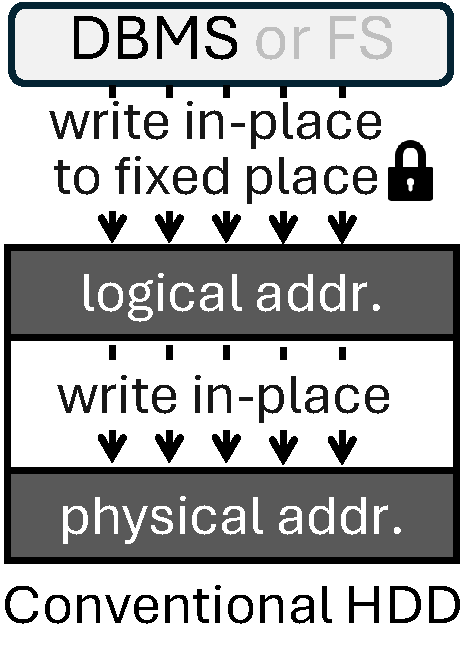
\includegraphics[width=0.6\linewidth]{figures/oopback0.pdf}
        \caption{In-place write on a conventional disk}
        \label{fig:oop0}
    \end{subfigure}
    \hfill
    \begin{subfigure}[b]{0.325\linewidth}
        \centering
        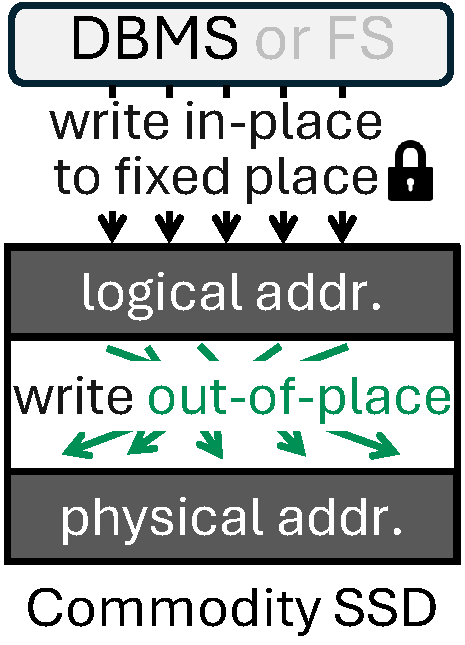
\includegraphics[width=0.6\linewidth]{figures/oopback1.pdf}
        \caption{In-place write on a commodity SSD}
        \label{fig:oop1}
    \end{subfigure}
    \hfill
    \begin{subfigure}[b]{0.325\linewidth}
        \centering
        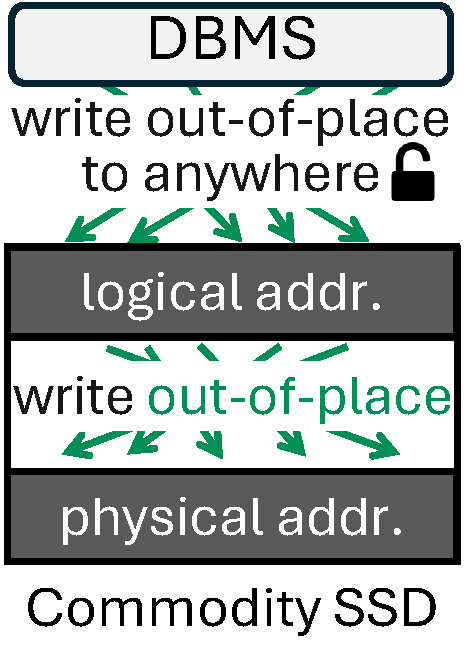
\includegraphics[width=0.6\linewidth]{figures/oopback2.pdf}
        \caption{Out-of-place write on a commodity SSD}
        \label{fig:oop2}
    \end{subfigure}
    \caption{In-place vs. out-of-place writes on disk and SSD}
    \vspace{-2mm} 
    \label{fig:oop}
\end{figure}

\module{Out-of-place writes are essential for minimizing total WAF.}
Even when a system aims to optimize SSD writes, the DBMS can do little if it performs in-place updates.
In-place systems fix each page’s file location (e.g., using the Page Identifier (PID) as an offset, as in \cref{fig:oop1}) and overwrite that location in the page size (16~KiB in InnoDB)~\cite{WObtree}.
Thus, the DBMS cannot alter write placement and therefore \emph{inherits} the device’s SSD WAF, forfeiting opportunities to optimize for SSDs.
Switching to out-of-place writes (\cref{fig:oop2}) unlocks flexibility, allowing the DBMS to group and place user writes as it chooses.
Out-of-place writes also eliminate doublewrite buffering: the old page remains valid until the new version is durably written, 
allowing crash recovery via the previous page and WAL replay.
Removing DWB nearly halves DB-issued bytes while preserving durability. 


\module{Joint consideration of DB and SSD WAF is necessary.}
\revision[R2.W1]{To optimize total WAF, the DBMS must account for both DB and SSD WAF and their interplay.
Focusing on only one layer can counterintuitively worsen the other.
For example, an LSM-tree engine can lower DB WAF by increasing size tiering~\cite{spooky}, but doing so consumes more SSD space and can raise SSD WAF, ultimately worsening total WAF.
Thus, total WAF---not individual components---must guide optimization, reflecting the effects of DBMS writes at both layers. }

\module{Unlocking optimizations that minimize total WAF.}
In the following sections, we propose several out-of-place-based optimizations that, taken together, minimize total WAF.
At the DBMS level, Page-wise Compression (\cref{sec:comppagepack}) and Deathtime-Based GC (\cref{sec:GDT}) reduce \emph{DB WAF} by lowering logical write volume.
At the device level, we present techniques that ensure \emph{SSD WAF~=~1} across all three SSD types: ZNS (\cref{sec:zns}), standard (\cref{sec:nowa}), and standard FDP-enabled SSDs (\cref{sec:fdp}).
To our knowledge, this is the first demonstration of SSD WAF~=~1 on commodity SSDs---even at 100\% utilization and without fully sequential workloads.
Although DB-side and SSD-side techniques must be applied together to minimize total WAF, individual optimizations may be selectively adopted depending on the device (e.g., SSD or disk) and integration layer (e.g., filesystem).
